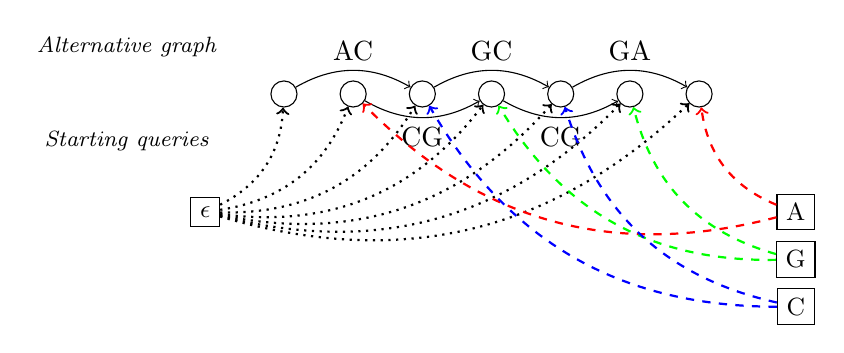
\begin{tikzpicture}[auto]
	\tikzstyle{state} = [ draw, circle, thin, node distance = 2.5em, font={\small}];
	\tikzstyle{query} = [ draw, rectangle, thin, node distance = 2.5em, font={\small}];
	\tikzstyle{info} = [font={\itshape\footnotesize}]
	\tikzstyle{point}  = [ ->, thin, font={\small}];
	\tikzstyle{extend} = [ ->, double, font={\small}];
	\tikzstyle{trace} = [ ->, thick, dashed, bend right, font={\small} ];


	\def \seq {X, A, C, G, C, G, A}

	\foreach \x [count=\xi] in \seq {
		\ifnum 1 < \xi
			\pgfmathparse{int(\xi-1)}
			\let \li \pgfmathresult
			\node[state, right of=\li] (\xi) {};
		\else
			\node[state] at(2,0) (\xi) {};
		\fi
	}

	\tikzstyle{labove} = [->, thin, bend left];
	\tikzstyle{lbelow} = [->, thin, bend right];

	\draw[labove] (1) to node[above]{AC} (3);
	\draw[lbelow] (2) to node[below]{CG} (4);
	\draw[labove] (3) to node[above]{GC} (5);
	\draw[lbelow] (4) to node[below]{CG} (6);
	\draw[labove] (5) to node[above]{GA} (7);

	\node[info] at (0,0.6) {Alternative graph};
	\node[info] at (0,-0.6) {Starting queries};

	\node[query](x) at (1,-1.5) {$\epsilon$};
	\node[query](A) at (8.5,-1.5) {A};
	\node[query](C) at (8.5,-2.7) {C};
	\node[query](G) at (8.5,-2.1) {G};

	\tikzstyle{tx} = [ ->, thick, dotted, bend right, color=black ];
	\tikzstyle{ta} = [ ->, thick, dashed, bend left, color=red ];
	\tikzstyle{tc} = [ ->, thick, dashed, bend left, color=blue ];
	\tikzstyle{tg} = [ ->, thick, dashed, bend left, color=green ];

	\draw[tx] (x) to (1);
	\draw[tx] (x) to (2);
	\draw[tx] (x) to (3);
	\draw[tx] (x) to (4);
	\draw[tx] (x) to (5);
	\draw[tx] (x) to (6);
	\draw[tx] (x) to (7);

	\draw[ta] (A) to (2);
	\draw[tc] (C) to (3);
	\draw[tg] (G) to (4);
	\draw[tc] (C) to (5);
	\draw[tg] (G) to (6);
	\draw[ta] (A) to (7);
\end{tikzpicture}
